%!TEX root = dissertation.tex

\chapter{Cuestionario complementario de la Actuación Avalada} \label{Ap:cuestionarioAA}

% the code below specifies where the figures are stored
\ifpdf
    \graphicspath{{Apendice/figures/PNG/}{Apendice/figures/PDF/}{Apendice/figures/}}
\else
    \graphicspath{{Apendice/figures/EPS/}{Apendice/figures/}}
\fi



\global\mdfdefinestyle{cuestionarioST}{%
linecolor=blue,linewidth=2pt,%
leftmargin=1cm,rightmargin=1cm
}

\global\mdfdefinestyle{hipotesis0}{%
linecolor=black,linewidth=1pt,%
leftmargin=1cm,rightmargin=1cm
}
Este apéndice contiene el cuestionario complementario que se envío a los docentes que participaron en la actuación avalada. Las secciones de este apéndice son:

\begin{itemize}
	\item Cuestionario (ver sección~\ref{apc:AA:cuestionario})
	\item Resultados  (ver sección~\ref{ape:AA:resultados})
\end{itemize}

\newpage

\section{Cuestionario} \label{apc:AA:cuestionario}

Los docentes que participaron en la actuación avalada recibieron un cuestionario complementario en la que marcaban para qué competencias genéricas considerarían los indicadores proporcionados por EvalCourse.

	\subsection*{A. Indicadores de accesos al campus virtual}

\begin{mdframed}[style=cuestionarioST]
		¿Qué competencia genérica podría evaluar con los indicadores de acceso al campus virtual?
			\begin{itemize}
				\item Trabajo en equipo
				\item Planificación y gestión del tiempo
				\item Razonamiento crítico y autocrítico
				\item Capacidad para identificar, plantear y resolver problemas
				\item Habilidades de interacción interpersonal
				\item Trabajo autónomo
				\item Otras
			\end{itemize}
		Explique o matice su respuesta si lo necesita y/o indique en qué otra competencia podría serle útil:\newline
			\rule{120mm}{1pt} 
\end{mdframed}

\newpage

	\subsection*{B. Indicadores de los foros}

\begin{mdframed}[style=cuestionarioST]
		¿Qué competencia genérica podría evaluar con los indicadores de los foros?
			\begin{itemize}
				\item Trabajo en equipo
				\item Planificación y gestión del tiempo
				\item Razonamiento crítico y autocrítico
				\item Capacidad para identificar, plantear y resolver problemas
				\item Habilidades de interacción interpersonal
				\item Trabajo autónomo
				\item Otras
			\end{itemize}
		Explique o matice su respuesta si lo necesita y/o indique en qué otra competencia podría serle útil:\newline
			\rule{120mm}{1pt}
\end{mdframed}

	\subsection*{C. Indicadores del wiki}

\begin{mdframed}[style=cuestionarioST]
		¿Qué competencia genérica podría evaluar con los indicadores del wiki?
			\begin{itemize}
				\item Trabajo en equipo
				\item Planificación y gestión del tiempo
				\item Razonamiento crítico y autocrítico
				\item Capacidad para identificar, plantear y resolver problemas
				\item Habilidades de interacción interpersonal
				\item Trabajo autónomo
				\item Otras
			\end{itemize}
		Explique o matice su respuesta si lo necesita y/o indique en qué otra competencia podría serle útil:\newline
			\rule{120mm}{1pt}
\end{mdframed}

	\subsection*{D. Indicadores de las actividades}

\begin{mdframed}[style=cuestionarioST]
		¿Qué competencia genérica podría evaluar con los indicadores de las actividades?
			\begin{itemize}
				\item Trabajo en equipo
				\item Planificación y gestión del tiempo
				\item Razonamiento crítico y autocrítico
				\item Capacidad para identificar, plantear y resolver problemas
				\item Habilidades de interacción interpersonal
				\item Trabajo autónomo
				\item Otras
			\end{itemize}
		Explique o matice su respuesta si lo necesita y/o indique en qué otra competencia podría serle útil:\newline
			\rule{120mm}{1pt}
\end{mdframed}

	\subsection*{E. Indicadores de los talleres}

\begin{mdframed}[style=cuestionarioST]
		¿Qué competencia genérica podría evaluar con los indicadores de los talleres?
			\begin{itemize}
				\item Trabajo en equipo
				\item Planificación y gestión del tiempo
				\item Razonamiento crítico y autocrítico
				\item Capacidad para identificar, plantear y resolver problemas
				\item Habilidades de interacción interpersonal
				\item Trabajo autónomo
				\item Otras
			\end{itemize}
		Explique o matice su respuesta si lo necesita y/o indique en qué otra competencia podría serle útil:\newline
			\rule{120mm}{1pt}
\end{mdframed}

\section{Resultados} \label{ape:AA:resultados}

	\subsection*{A. Indicadores de accesos al campus virtual}

El número de docentes que consideraría utilizar los indicadores de acceso al campus virtual para cada competencias genérica puede verse en la figura~\ref{fig:ape:aa:accesos}.

\begin{figure}[ht]
    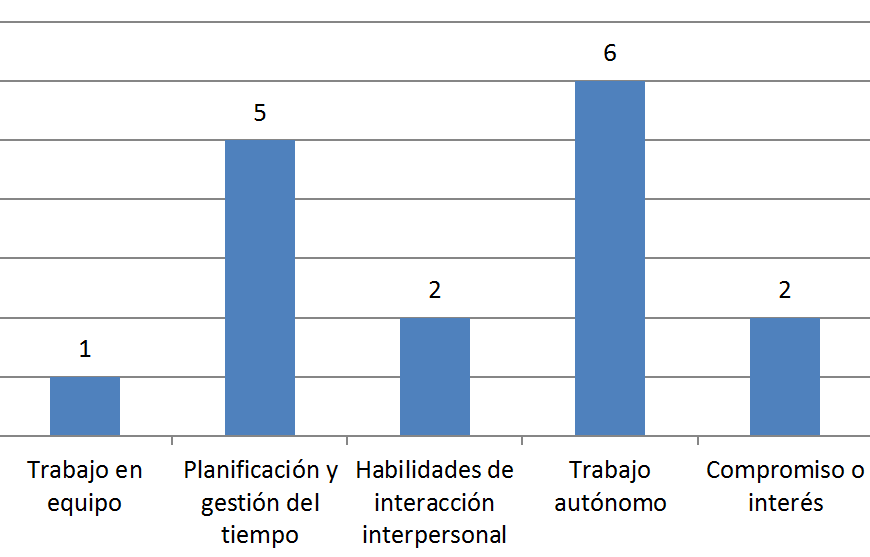
\includegraphics[scale=0.45]{aa_accesos.png}
  \caption{Docentes que considerarían los indicadores de accesos para evaluar cada competencia genérica de una población de 7}
  \label{fig:ape:aa:accesos}
\end{figure}

\paragraph*{Comentarios}

\begin{itemize}
\item Interés por la asignatura. El interés y participación de los alumnos cambia drásticamente de un grado a otro e incluso de una facultad a otra. En la asignatura analizada del grado de Publicidad y Relaciones Públicas, impartido en la Facultad de Ciencias Sociales y de la Comunicación del Campus de Jerez parece que no son muy dados a visualizar y/o participar en el campus virtual de una asignatura, de hecho hay que fomentar su participación haciendo que ésta forme parte de la evaluación de la misma (mínimo un 10\percentage). Con este indicador, conociendo el número de días que se imparte la asignatura y obteniendo el número de veces que acceden al campus virtual, se puede determinar quiénes son alumnos muy activos, bastante activos, activos, poco activos y nada activos en la asignatura. Pudiéndose así evaluar el interés que puedan tener por la misma.
\item Un mayor número de accesos al campus podría indicar quizás, grado de compromiso o interés.
\item Es interesante observar la idoneidad del siguiente planteamiento: las capacidades de planificación y gestión de tiempo siguen una curva gaussiana desplazada hacia un menor número de accesos al campus, teniendo en cuenta factores como la participación práctica. Es decir, que una persona que accede muchas veces no necesariamente se planifica bien; diría que es al contrario.
\item Planificación y gestión del tiempo, siempre y cuando se proporcionase el número de accesos por día, semana, etc.
\end{itemize}

	\subsection*{B. Indicadores de los foros}

El número de docentes que consideraría utilizar los indicadores de acceso al campus virtual para cada competencias genérica puede verse en la figura~\ref{fig:ape:aa:foros}.

\begin{figure}[ht]
    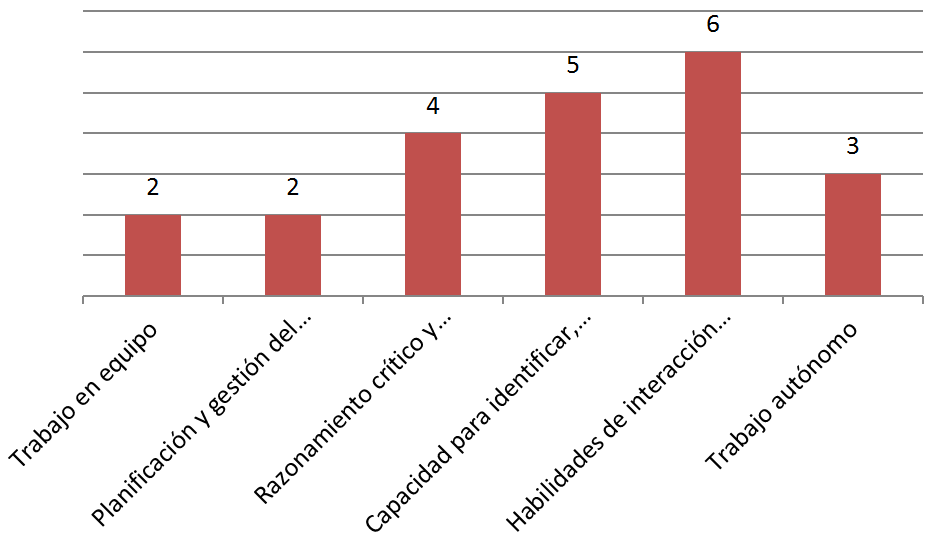
\includegraphics[scale=0.4]{aa_foros.png}
  \caption{Docentes que considerarían los indicadores de los foros para evaluar cada competencia genérica de un máximo}
  \label{fig:ape:aa:foros}
\end{figure}

\paragraph*{Comentarios}

\begin{itemize}
\item Uno de los foros de la asignatura se emplea para que los alumnos publiquen novedades, noticias, tutoriales, etc que sean de interés para la asignatura. Los alumnos identifican ``elementos'' que estén relacionados con la materia: bien sean noticias como tutoriales que puedan resolver algún problema práctico de la asignatura. Del mismo modo se plantean cuestiones al resto de compañeros fomentando la interacción interpersonal.
\item La capacidad para identificar, plantear y resolver problemas sería posible marcarla si se analizara el contenido de los foros. Podemos suponer que una persona que responde puede resolver problemas, pero la identificación y el planteamiento no queda claro.
\end{itemize}

	\subsection*{C. Indicadores del wiki}

El número de docentes que consideraría utilizar los indicadores de acceso al campus virtual para cada competencias genérica puede verse en la figura~\ref{fig:ape:aa:wikis}.

\begin{figure}[ht]
	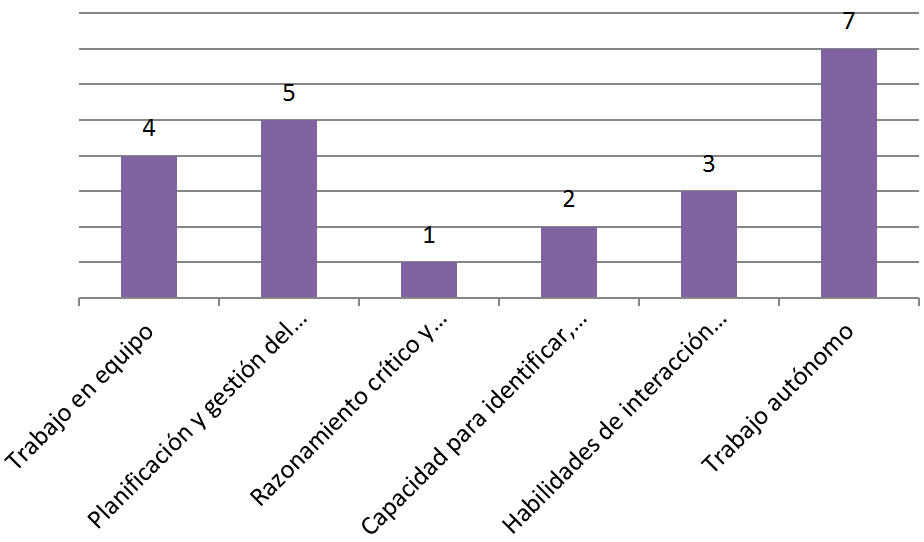
\includegraphics[scale=0.35]{aa_wikis.png}
	\caption{Docentes que considerarían los indicadores de los wikis para evaluar cada competencia genérica de un máximo de 7}
	\label{fig:ape:aa:wikis}
\end{figure}


\paragraph*{Comentarios}

\begin{itemize}
\item El wiki de los alumnos es un wiki individual para el seguimiento de una de las actividades a entregar. Cada vez que terminaban un paso del proyecto, iban completando una parte del wiki. Tenían todo el semestre para ir completando la actividad y wiki, lo que permite evaluar perfectamente cómo se ha planificado cada alumno en el curso, la capacidad para resolver los problemas y el trabajo autónomo del alumno.
\item No me quedan claro lo que representan los ejes de las gráficas. Entiendo que se refiere a la cantidad de contribuciones (ordenadas) por semanas (abscisas). Refiero lo mismo en relación a la gestión del tiempo: no todo el que colabora mucho se gestiona de forma práctica. De hecho, un alumno ``práctico'' debería saber optimizar su tiempo, y generalmente la participación en una Wiki es superflua (salvo límites obligatorios). Las inquietudes personales y la autoexigencia está muy relacionados con el rendimiento, pero no necesariamente con las habilidades. Esto es extensible al resto de los datos.
\end{itemize}

	\subsection*{D. Indicadores de las actividades}

El número de docentes que consideraría utilizar los indicadores de acceso al campus virtual para cada competencias genérica puede verse en la figura~\ref{fig:ape:aa:actividades}.

\begin{figure}[ht]
    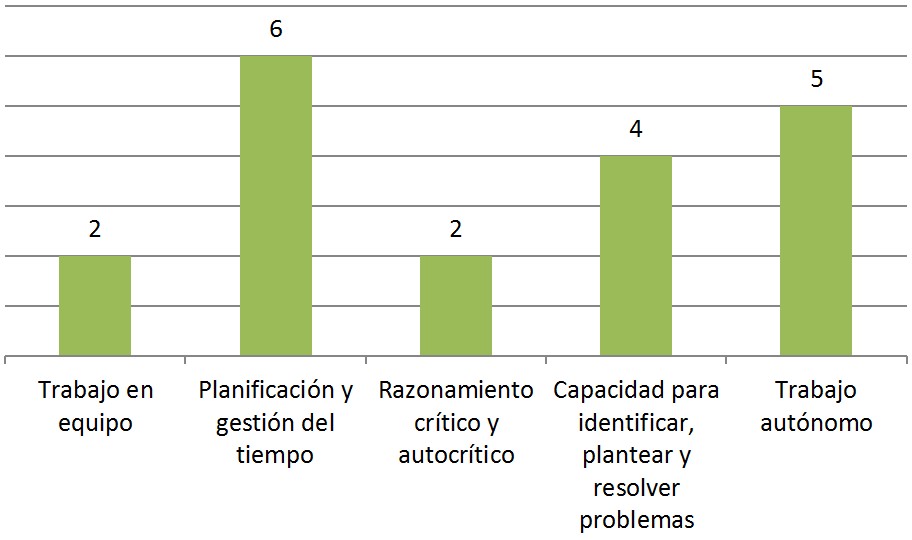
\includegraphics[scale=0.4]{aa-actividades.png}
  \caption{Docentes que considerarían los indicadores de las actividades para evaluar cada competencia genérica de un máximo de 7}
  \label{fig:ape:aa:actividades}
\end{figure}

\paragraph*{Comentarios}

\begin{itemize}
\item Las actividades a entregar en la asignatura eran de carácter individual, luego el hecho de la entrega de las mismas a tiempo permite evaluar perfectamente la planificación de los alumnos que la entregan (algunas actividades tenían una entrega optativa). En una de las actividades (optativas), en la que no se le facilitaban todos los pasos, permite evaluar que los alumnos han intentado identificar y resolver los problemas planteados y por supuesto, los que han participado, han fomentado su trabajo autónomo en la asignatura.
\item Si se proponen actividades en grupo, éstas podrían medir el trabajo en equipo.
\item Planificación y gestión del tiempo, se presupone que es posible acabar las tareas en un tiempo razonable sin ``quemar'' al alumno.
\item Trabajo en equipo, siempre y cuando se considere en los resultados las tareas con la opción de Moodle de ``entrega por grupo''. 
\end{itemize}

	\subsection*{E. Indicadores de los talleres}

Sólo hubo una profesora que utilizó los talleres y en concreto los consideró para evaluar las competencias de la capacidad para  identificar, plantear y resolver problemas, las habilidades de interacción interpersonal y el trabajo autónomo.
